\documentclass[11pt,a4paper]{article}
\usepackage[T1]{fontenc}
\usepackage[margin=2.3cm]{geometry}
\usepackage{amsmath,amssymb}
\usepackage{graphicx}
\usepackage[dvipsnames]{xcolor}
\usepackage{enumitem}
\usepackage[colorlinks=true,linkcolor=blue,urlcolor=blue]{hyperref}
\setlength{\parskip}{0.6em}
\setlength{\parindent}{0pt}
\begin{document}

\begin{center}{\LARGE\bfseries openincline}\\[0.4em]{\large Find the angle where a block starts to slide, in three sessions.}\\[0.2em]\small PAN IIT OSS explainer \textbullet{} secondary school to diploma / undergraduate (levels 3-5)\end{center}

\section*{Why this exists}
A block on a ramp is the simplest picture in which gravity, a supporting surface and friction all matter. This explainer follows the forces from the free-body diagram to a simulation that you can check against exact answers.

\section*{The end goal}
Find the angle where a block starts to slide on a ramp. The end goal is to find, by calculation and by simulation, the angle where a block first starts to slide on a ramp, and to say how sure you are. The same reasoning applies to the grip of tyres, the holding of screws and the stability of soil slopes, each of which needs far more care in real design.

\section*{How the three sessions build up}
\begin{enumerate}[nosep]
\item \textbf{Session 1: Forces on a ramp: friction is a limit} (Level 1, conceptual interactive model, 60 min).
\item \textbf{Session 2: The equations: static and kinetic friction} (Level 2, mathematical engineering model, 75 min).
\item \textbf{Session 3: Simulating the block and validating it} (Level 3, simulation and validation, 90 min).
\end{enumerate}

\section{Session 1: Forces on a ramp: friction is a limit}

\subsection*{A. Real-world problem}
A parked car on a hill, a box on a loading ramp, a book on a tilted desk. Tilt the surface a little and nothing moves; tilt it more and suddenly it slides. What decides the angle where the sliding starts? Does a heavier block need a steeper ramp? (This is a simplified model for learning, not a design tool for real ramps or vehicles.)

\subsection*{B. Concept and theory}
The weight m g points straight down. On a ramp tilted by an angle t it is easier to use two directions: perpendicular to the ramp, where the ramp pushes back with the normal force N, and along the slope, where the pull F tries to make the block slide. Friction acts up the slope and opposes sliding. It is not a fixed number: it matches the pull exactly, up to a largest value mu times N, where mu (the friction coefficient) has no unit and depends on the two surfaces. If the pull is below the limit nothing moves; if it would exceed the limit the block accelerates. Comparing m g sin t with mu m g cos t, the mass cancels, leaving the slide condition tan t \textgreater{} mu.

\begin{itemize}[nosep]
\item m: mass of the block (kg)
\item g: gravity (9.81) (m/s\textasciicircum{}2)
\item t: ramp angle from the horizontal (degrees)
\item N: normal force, perpendicular to the ramp (N)
\item F: pull of gravity along the slope (N)
\item mu: friction coefficient (one value for Session 1) (no unit)
\item f: friction force that actually acts (N)
\item a: acceleration down the slope (m/s\textasciicircum{}2)
\end{itemize}

\begin{equation*}
N=mg\cos\theta,\qquad F=mg\sin\theta
\end{equation*}

\begin{equation*}
f_{\max}=\mu N=\mu mg\cos\theta,\qquad f=\min(F,\ \mu N)
\end{equation*}

\begin{equation*}
\text{slides if } mg\sin\theta>\mu mg\cos\theta\iff \tan\theta>\mu,\qquad a=\frac{F-f}{m}
\end{equation*}

\begin{center}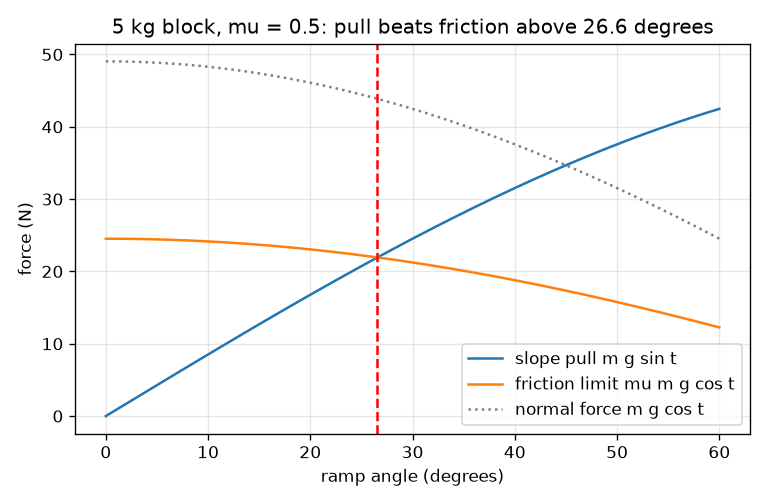
\includegraphics[width=0.85\linewidth]{figures/s01_forces_vs_angle.png}\\\small Slope pull rises and the friction limit falls; they cross at the slide angle (26.6 degrees for mu = 0.5).\end{center}

\subsection*{E. Worked example}
A 5 kg block rests on a ramp at 20 degrees with mu = 0.5. Find N, the slope pull and the friction limit. Does it hold? At what angle would it begin to slide?
\begin{enumerate}[nosep]
\item N = m g cos t = 5 * 9.81 * cos 20 = 5 * 9.81 * 0.9397 = 46.09 N.
\item Pull F = m g sin t = 5 * 9.81 * 0.3420 = 16.78 N.
\item Friction limit = mu N = 0.5 * 46.09 = 23.05 N.
\item The pull 16.78 N is below the limit 23.05 N, so the block holds: friction equals 16.78 N and the net force is 0.
\item The slide angle solves tan t = mu = 0.5, so t = arctan 0.5 = 26.57 degrees. Check: tan 20 = 0.364 \textless{} 0.5, consistent with holding.
\end{enumerate}
\textbf{Answer.} N = 46.09 N, pull = 16.78 N, limit = 23.05 N; the block holds with 16.78 N of friction. It starts to slide above 26.57 degrees, whatever its mass.

\subsection*{F. Questions}
\begin{enumerate}[nosep]
\item \textbf{Conceptual.} What determines whether a block at rest on a ramp begins to slide? Does the mass matter? Does the size of the block's bottom face matter?
\item \textbf{Numerical.} An 8 kg block sits on a ramp at 15 degrees, mu = 0.35. Find N, the pull, the friction limit and the friction that acts. Does it slide? Sanity check the answer.
\item \textbf{Graph and simulation interpretation.} On the force graph for a 5 kg block, the slope pull and the friction limit cross at 26.6 degrees for mu = 0.5. Where would they cross for mu = 0.8, and which curve moves? What does the friction curve do to the left of the crossing?
\item \textbf{Design and optimisation challenge.} Design: a 20 kg box must stay put without a rope on a wooden ramp with mu = 0.45. Pick a maximum ramp angle with a safety margin, so that the friction needed is at most 80 percent of the limit. A 1.2 m rise is needed. How long must the ramp be? What is the trade-off?
\end{enumerate}

\section{Session 2: The equations: static and kinetic friction}

\subsection*{A. Real-world problem}
A warehouse wants crates to slide down a ramp by themselves and reach the bottom at a gentle, known speed. If the ramp is too shallow the crate never starts; too steep and it arrives too fast. The surface decides the friction. Which angle should the ramp have to make a crate slide 3 m in 2 seconds? (Simplified model; real crate handling needs a professional safety assessment.)

\subsection*{B. Concept and theory}
A block at rest is held by static friction, which can be as large as mu\_s N. Once the block slides, kinetic friction acts with a constant size mu\_k N, usually a little smaller (mu\_k \textless{}= mu\_s). While the block holds, friction equals the pull and the net force is zero. The block starts as soon as tan t \textgreater{} mu\_s. After that Newton's second law along the slope, m a = m g sin t - mu\_k m g cos t, gives an acceleration that does not depend on the mass. From rest with constant a, speed is v = a t and distance x = (1/2) a t\textasciicircum{}2. Because friction drops from its limit mu\_s N to mu\_k N when slipping starts, the acceleration jumps from 0 to a positive value instead of growing smoothly.

\begin{itemize}[nosep]
\item mu\_s: static friction coefficient (no unit)
\item mu\_k: kinetic friction coefficient (mu\_k \textless{}= mu\_s) (no unit)
\item t: ramp angle (degrees)
\item a: acceleration down the slope (m/s\textasciicircum{}2)
\item v: speed after time T (m/s)
\item x: distance travelled from rest (m)
\item T: time since release (s)
\end{itemize}

\begin{equation*}
\text{holds if } \tan\theta\le\mu_s,\qquad \theta_{\text{slide}}=\arctan\mu_s
\end{equation*}

\begin{equation*}
a=g\,(\sin\theta-\mu_k\cos\theta)
\end{equation*}

\begin{equation*}
v=aT,\qquad x=\tfrac12 aT^2
\end{equation*}

\begin{equation*}
\theta=\arctan\mu_k+\arcsin\!\left(\frac{a}{g\sqrt{1+\mu_k^2}}\right)
\end{equation*}

\begin{center}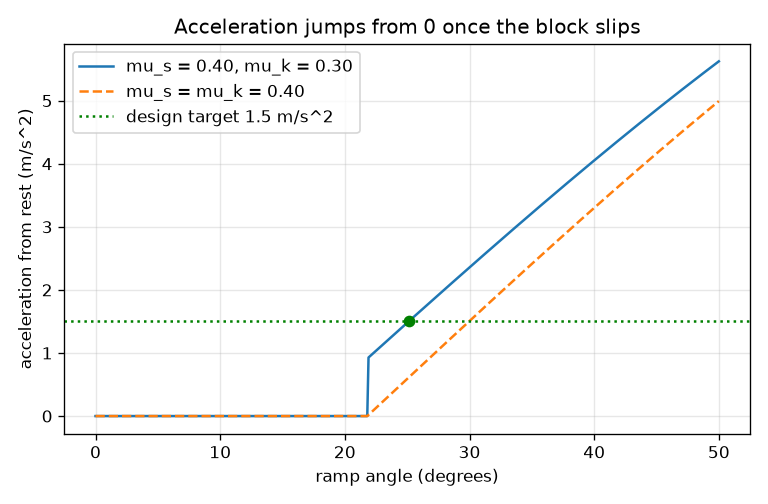
\includegraphics[width=0.85\linewidth]{figures/s02_accel_vs_angle.png}\\\small Acceleration from rest: zero until 21.8 degrees, then a jump; the green dot is the design point.\end{center}

\subsection*{E. Worked example}
A 10 kg crate is released from rest on a ramp at 30 degrees with mu\_s = 0.40 and mu\_k = 0.30. Does it slide? Find the friction, the acceleration, and the speed and distance after 2 s.
\begin{enumerate}[nosep]
\item tan 30 = 0.577 \textgreater{} mu\_s = 0.40, so the crate slides (the slide angle is arctan 0.40 = 21.80 degrees).
\item N = 10 * 9.81 * cos 30 = 84.96 N; kinetic friction = 0.30 * 84.96 = 25.49 N (the static limit would have been 33.98 N).
\item Pull = 10 * 9.81 * sin 30 = 49.05 N, so net force = 49.05 - 25.49 = 23.56 N and a = 23.56 / 10 = 2.356 m/s\textasciicircum{}2.
\item Check with the formula: a = 9.81 * (0.5 - 0.30 * 0.8660) = 2.356 m/s\textasciicircum{}2; the mass cancelled.
\item After 2 s: v = 2.356 * 2 = 4.71 m/s and x = 0.5 * 2.356 * 4 = 4.71 m.
\end{enumerate}
\textbf{Answer.} The crate slides with a = 2.356 m/s\textasciicircum{}2; after 2 s it moves at 4.71 m/s and has travelled 4.71 m.

\subsection*{F. Questions}
\begin{enumerate}[nosep]
\item \textbf{Conceptual.} Why does a block often 'jerk' into motion rather than speeding up smoothly from rest? What happens to the friction force at the moment of slipping?
\item \textbf{Numerical.} A 4 kg block is released at 35 degrees with mu\_s = 0.5 and mu\_k = 0.4. Does it slide? Find the friction force and the acceleration. Show a sanity check.
\item \textbf{Graph and simulation interpretation.} On the acceleration graph for mu\_s = 0.40 and mu\_k = 0.30, what is the acceleration just above the slide angle? Why is the graph not a smooth curve starting at 0?
\item \textbf{Design and optimisation challenge.} Design: choose the ramp angle (whole degrees) so that a crate with mu\_s = 0.40 and mu\_k = 0.30 slides 3 m in 2 s. Check it starts. How high is the top of a 3 m long ramp? What goes wrong if the surface had mu\_k = 0.20 but mu\_s = 0.40?
\end{enumerate}

\section{Session 3: Simulating the block and validating it}

\subsection*{A. Real-world problem}
To measure a friction coefficient you tilt a board slowly until the block slips, but you cannot see the exact instant and the coefficient is never known exactly. Before trusting a model, an engineer checks that the simulation reproduces cases with a known exact answer, and asks how much an uncertain input changes the result. Can we simulate the tilting test, check it, and decide how precisely mu\_s must be known? (Educational model only, not a validated tool for real ramps or vehicles.)

\subsection*{B. Concept and theory}
Cut time into small steps dt. In the stuck state the block does not move until the pull m g sin t exceeds the static limit mu\_s m g cos t; then it switches to sliding. In the sliding state a = g (sin t - mu\_k cos t); position and speed are advanced by x + v dt + (1/2) a dt\textasciicircum{}2 and v + a dt, and if the speed would turn negative the block stops and is stuck again. The ramp angle can change in time, so the simulation can tilt the ramp slowly as in the real test. Validation compares the output with exact references. Because tan t = mu\_s, a small error d(mu) in mu\_s changes the slide angle by d(mu) / (1 + mu\textasciicircum{}2) radians. A body that rolls without slipping also spins, so its acceleration is g sin t / (1 + k) with k = I / (m r\textasciicircum{}2): k = 1/2 for a solid cylinder and 1 for a hollow tube. Friction does no work on a rolling body; it only needs to be large enough: mu\_s \textgreater{}= tan t * k / (1 + k).

\begin{itemize}[nosep]
\item dt: time step (s)
\item theta(t): ramp angle as a function of time (degrees)
\item x, v: position and speed down the slope (m, m/s)
\item d(mu): uncertainty of mu\_s (no unit)
\item I: moment of inertia of the rolling body about its axis (kg m\textasciicircum{}2)
\item k: I / (m r\textasciicircum{}2), the shape factor of the rolling body (no unit)
\item r: radius of the rolling body (m)
\end{itemize}

\begin{equation*}
x_{n+1}=x_n+v_n\,\Delta t+\tfrac12 a\,\Delta t^2,\qquad v_{n+1}=v_n+a\,\Delta t
\end{equation*}

\begin{equation*}
\theta_{\text{slip}}=\arctan\mu_s,\qquad \Delta\theta\approx\frac{\Delta\mu}{1+\mu_s^2}\ \text{(radians)}
\end{equation*}

\begin{equation*}
a_{\text{roll}}=\frac{g\sin\theta}{1+I/(mr^2)},\qquad \mu_s\ge\tan\theta\,\frac{k}{1+k}
\end{equation*}

\begin{center}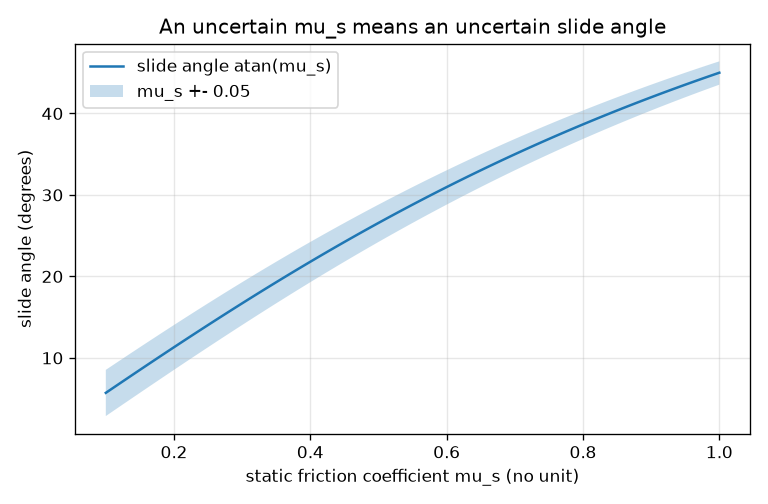
\includegraphics[width=0.85\linewidth]{figures/s03_sensitivity.png}\\\small Slide angle against mu\_s with a +-0.05 uncertainty band.\end{center}

\subsection*{E. Worked example}
Simulate a block at a fixed 30 degrees with mu\_s = 0.40 and mu\_k = 0.30 for 2 s. Compare with the exact distance, then find how a 0.05 uncertainty in mu\_s = 0.5 moves the slide angle.
\begin{enumerate}[nosep]
\item tan 30 = 0.577 \textgreater{} 0.40, so the simulation switches to sliding immediately.
\item Exact a = 9.81 * (sin 30 - 0.30 * cos 30) = 2.356 m/s\textasciicircum{}2, so exact x(2 s) = 0.5 * 2.356 * 4 = 4.71 m and v = 4.71 m/s.
\item The simulation with dt = 0.001 s gives the same x(t) to within 1e-6 m over the whole 2 s, because the update rule is exact for constant acceleration.
\item Tilting test with mu\_s = 0.5: the simulation slips at 26.566 degrees against the exact arctan 0.5 = 26.565 degrees.
\item Sensitivity: mu\_s = 0.45 gives arctan 0.45 = 24.23 degrees and mu\_s = 0.55 gives 28.81 degrees, a spread of 4.58 degrees, or about +-2.3 degrees; the linear formula 0.05 / 1.25 rad = 2.29 degrees agrees.
\end{enumerate}
\textbf{Answer.} Simulated and exact motion agree (4.71 m after 2 s, error below 1e-6 m); the simulated slide angle is 26.57 degrees, as arctan 0.5; a 0.05 uncertainty in mu\_s = 0.5 gives about +-2.3 degrees in the slide angle.

\subsection*{F. Questions}
\begin{enumerate}[nosep]
\item \textbf{Conceptual.} Why does the simulation need a 'stuck' state? What would go wrong if it always used kinetic friction?
\item \textbf{Numerical.} A block has mu\_s = 0.30 with an uncertainty of +-0.03. Find the range of its slide angle. Compare with the linear estimate.
\item \textbf{Graph and simulation interpretation.} In the slow-tilt figure the block does not move until about 53 s. Why 53 s? What would you see if the tilt rate were doubled to 1 degree per second?
\item \textbf{Design and optimisation challenge.} Design: a 2 m ramp at 20 degrees must deliver a rolling barrel to the bottom in at least 1.5 s so that the barrel does not hit the stop too hard. Compare a solid cylinder (k = 0.5) and a hollow tube (k = 1.0). Which satisfies the limit, and what friction coefficient is needed to avoid slipping?
\end{enumerate}

\section{Real-world mini-project}
\textbf{Measure the friction coefficient with a board and a phone.} Put a block (a book, a wooden block, an eraser) on a flat board. Lift one end slowly while a phone angle app lies on the board and shows the tilt; note the angle at which the block first starts to slip. Repeat at least 10 times, wiping the surfaces each time, and then try a second surface (sandpaper or cloth). You do not need a ramp to begin: \texttt{synthetic\_tilt\_trials()} in Session 3 makes made-up data, and the lesson saves it as \texttt{ramp\_trials.csv} (columns trial and slip\_angle\_deg) so you can test your analysis first. Safety: keep fingers clear and use a soft landing area. Use only objects that are safe to drop.

\section{The path ahead}
\begin{enumerate}[nosep]
\item \textbf{Session 4: Slide angle on a curved surface.} A simulation of a block on a hill profile y(x) with friction, finding where it can stay.
\item \textbf{Session 5: Stick-slip: a block pulled by a spring.} A block on a surface pulled through a spring by a slowly moving end.
\item \textbf{Session 6: A phase map of stick versus slide.} A map over (angle, friction coefficient) coloured by the simulated outcome.
\item \textbf{Session 7: Tip or slide: finite block size.} A block with a centre of mass height h and base width w on a ramp.
\item \textbf{Session 8: Rolling with slipping.} A solid cylinder on a steep ramp with low friction.
\end{enumerate}

\section{Answers and hints}

\subsection*{Session 1}
\begin{enumerate}[nosep]
\item \textbf{Conceptual.} Hint: Compare m g sin t with mu m g cos t. What cancels? Solution: Only the angle and the friction coefficient of the two surfaces decide: the block slides when tan t is larger than mu. The mass m appears in both the pull and the friction limit and cancels, so a heavy and a light block of the same material start to slide at the same angle. In the simple friction law the contact area does not matter either: a bigger face spreads the same N over more area but the limit mu N is unchanged.
\item \textbf{Numerical.} Hint: Use N = m g cos t, F = m g sin t, limit = mu N, then compare. Solution: N = 8 * 9.81 * cos 15 = 75.81 N. F = 8 * 9.81 * sin 15 = 20.31 N. Limit = 0.35 * 75.81 = 26.53 N. Since 20.31 \textless{} 26.53 the block holds and the friction that acts is 20.31 N. Check: the slide angle is arctan 0.35 = 19.29 degrees, above 15 degrees, so holding is right. Units: newtons.
\item \textbf{Graph and simulation interpretation.} Hint: Only the friction-limit curve contains mu. Solve tan t = 0.8. Solution: The red friction-limit curve scales up with mu, so it moves up and the crossing moves right to arctan 0.8 = 38.66 degrees. The pull curve does not contain mu and stays put. To the left of the crossing the limit is above the pull, so the block holds there; to the right the pull is larger and the block slides.
\item \textbf{Design and optimisation challenge.} Hint: The friction needed is the pull, so F \textless{}= 0.8 * mu N means tan t \textless{}= 0.8 mu. Length = rise / sin t. Solution: tan t \textless{}= 0.8 * 0.45 = 0.36, so t \textless{}= 19.80 degrees (the slide angle is 24.23 degrees). Ramp length = 1.2 / sin 19.80 = 3.54 m. At the slide angle it would be only 2.92 m but with no safety margin. The trade-off is space against safety: a gentler, longer ramp is safer if the surface gets wet or dusty and mu drops. The mass of 20 kg does not change the answer. This is a classroom model; real ramps need professional design.
\end{enumerate}

\subsection*{Session 2}
\begin{enumerate}[nosep]
\item \textbf{Conceptual.} Hint: Compare the static limit mu\_s N with kinetic friction mu\_k N. Solution: Static friction can grow up to mu\_s N, but once the block slips only kinetic friction mu\_k N acts, and mu\_k is usually smaller. The friction force therefore drops suddenly at the slip angle, so the net force down the slope jumps from zero to a positive value and the acceleration jumps with it. The bigger the gap between mu\_s and mu\_k, the stronger the jerk (this is also behind stick-slip squeaks).
\item \textbf{Numerical.} Hint: Compare tan 35 with mu\_s first, then use a = g (sin t - mu\_k cos t). Solution: tan 35 = 0.700 \textgreater{} 0.5, so it slides. Kinetic friction = 0.4 * 4 * 9.81 * cos 35 = 12.86 N; the pull is 4 * 9.81 * sin 35 = 22.51 N. a = 9.81 * (0.5736 - 0.4 * 0.8192) = 2.412 m/s\textasciicircum{}2. Check: net force 22.51 - 12.86 = 9.65 N divided by 4 kg = 2.41 m/s\textasciicircum{}2. Units: m/s\textasciicircum{}2.
\item \textbf{Graph and simulation interpretation.} Hint: Evaluate g (sin t - mu\_k cos t) at 22 degrees. Solution: At 22 degrees a = 9.81 * (0.3746 - 0.30 * 0.9272) = 0.946 m/s\textasciicircum{}2, so the graph jumps from 0 to about 0.95 m/s\textasciicircum{}2 at 21.8 degrees. It is not smooth because the friction force drops from mu\_s N to mu\_k N when slipping starts; if mu\_k equalled mu\_s the curve would start smoothly from zero.
\item \textbf{Design and optimisation challenge.} Hint: Needed a = 2 * 3 / 2\textasciicircum{}2 = 1.5 m/s\textasciicircum{}2. Solve numerically or use theta = arctan(mu\_k) + arcsin(a / (g sqrt(1 + mu\_k\textasciicircum{}2))). Solution: a = 1.5 m/s\textasciicircum{}2 gives t = 25.12 degrees; whole degrees: 25 degrees gives a = 1.479 m/s\textasciicircum{}2, 2.96 m in 2 s and a final speed of 2.96 m/s. It starts because tan 25 = 0.466 \textgreater{} 0.40. Height of a 3 m ramp = 3 * sin 25 = 1.27 m. With mu\_k = 0.20 the formula gives 19.9 degrees, but that is below the slide angle 21.8 degrees, so the crate would never start: the design needs both the angle for the acceleration and the check tan t \textgreater{} mu\_s. Trade-off: the margin above the slide angle is only about 3 degrees, so a rougher surface could stop the crate; a slightly steeper ramp is more robust but faster.
\end{enumerate}

\subsection*{Session 3}
\begin{enumerate}[nosep]
\item \textbf{Conceptual.} Hint: What does a = g (sin t - mu\_k cos t) give for a block that is held by static friction? Solution: Below the slide angle the block holds, with friction equal to the pull. Using the sliding formula with mu\_k would give a positive acceleration whenever tan t \textgreater{} mu\_k, so the simulated block would creep or slide at angles where a real block stays put, and the slip angle would come out as arctan(mu\_k) instead of arctan(mu\_s). The stuck state with the static limit is what reproduces the right slide angle.
\item \textbf{Numerical.} Hint: Use arctan(0.27) and arctan(0.33). The linear estimate is d(mu) / (1 + mu\textasciicircum{}2) in radians. Solution: arctan 0.27 = 15.11 degrees and arctan 0.33 = 18.26 degrees, so the slide angle is 16.70 degrees with a range of about +-1.6 degrees. Linear estimate: 0.03 / (1 + 0.09) = 0.0275 rad = 1.58 degrees. They agree; the symmetric range is a good approximation for small d(mu).
\item \textbf{Graph and simulation interpretation.} Hint: Time = angle / rate. Which angle? Solution: The slip angle for mu\_s = 0.5 is 26.57 degrees, and at 0.5 degrees per second the ramp reaches it after 26.57 / 0.5 = 53.1 s. At twice the rate the block slips at the same angle, after 26.6 s: the slip angle does not depend on the rate in the model (the simulation at 5 degrees per second still gives 26.57 degrees, with a small delay of one time step).
\item \textbf{Design and optimisation challenge.} Hint: a = g sin t / (1 + k), time = sqrt(2 d / a), and mu\_s \textgreater{}= tan t * k / (1 + k). Solution: At 20 degrees: solid cylinder a = 2.237 m/s\textasciicircum{}2, time = 1.337 s (too fast); hollow tube a = 1.678 m/s\textasciicircum{}2, time = 1.544 s (meets the limit). A frictionless block would take only 1.092 s. The hollow tube needs mu\_s \textgreater{}= tan 20 * 0.5 = 0.182 to roll without slipping, so choose a surface with mu\_s of 0.25 or more for a margin. Trade-off: a more massive rim slows the descent but needs more friction to avoid slipping at steeper angles.
\end{enumerate}

\section{How to join}
Read \texttt{CONTRIBUTING.md} in the repository, then pick an issue labelled \texttt{good first issue}. Repository: \url{https://github.com/KrunalPanchal1995/openincline}

\end{document}
